\documentclass[12pt, letterpaper]{article}  % change to >11 pt if you like, and change article with report
\usepackage[letterpaper, top=3.71cm, bottom=3.20cm, left=2.86cm, right=2.86cm]{geometry}
%top = 2.44 (header in doc) + 1.27
% bottom 1.42 (footer in doc) + 1.78
\usepackage[utf8]{inputenc}
\usepackage{natbib}
\usepackage{graphicx}
\usepackage{color}
\usepackage{algorithm}
\usepackage{algpseudocode}
\usepackage{multirow}

\DeclareMathAlphabet{\mathcal}{OMS}{cmsy}{m}{n}
\SetMathAlphabet{\mathcal}{bold}{OMS}{cmsy}{b}{n}

\newcommand{\bigO}{\mathcal{O}}
\renewcommand\refname{} %remove this line to automatically show the bibliography header

\begin{document}
\nocite{*}  % comment this line to list only the articles you really cite

\begin{titlepage}

\newcommand{\HRule}{\rule{\linewidth}{0.5mm}} % Defines a new command for the horizontal lines, change thickness here

\center % Center everything on the page
 
%----------------------------------------------------------------------------------------
%	HEADING SECTIONS
%----------------------------------------------------------------------------------------

\textsc{\LARGE Università di Pisa}\\[1.5cm] % Name of your university/college
\textsc{\Large Computer Science Master Degree}\\[0.5cm] % Major heading such as course name
%\textsc{\large Assignment 1}\\[0.5cm] % Minor heading such as course title

%----------------------------------------------------------------------------------------
%	TITLE SECTION
%----------------------------------------------------------------------------------------

\HRule \\[0.75cm]
{ \huge \bfseries Implementing KNN using C\verb!++! threads and Fastflow}\\[0.4cm] % Title of your document
\HRule \\[1.5cm]
 
%----------------------------------------------------------------------------------------
%	AUTHOR SECTION
%----------------------------------------------------------------------------------------

\large
\emph{Author:} Dario \textsc{SALVATI} \\
\emph{Mat:} 619628

\vspace{2cm}

% If you don't want a supervisor, uncomment the two lines below and remove the section above
%\Large \emph{Author:}\\
%John \textsc{Smith}\\[3cm] % Your name

%----------------------------------------------------------------------------------------
%	DATE SECTION
%----------------------------------------------------------------------------------------

{\large ACADEMIC YEAR 2020/2021}\\[2cm] % Date, change the \today to a set date if you want to be precise

%----------------------------------------------------------------------------------------
%	LOGO SECTION
%----------------------------------------------------------------------------------------


\includegraphics[width=140px, keepaspectratio]{imgs/university.png}\\[1cm] % Include a department/university logo - this will require the graphicx package
 
%----------------------------------------------------------------------------------------

\vfill % Fill the rest of the page with whitespace

\end{titlepage}

\newpage

\begin{abstract}
    K-Nearest Neighbors is a non-parametric classification method used mainly to label elements of a multi-dimensional space. The class assigned to each point is based on the plurality vote of its neighbors. In this report I'll discuss how I implemented the algorithm using C\verb!++! threads and also using the Fastflow framework, in order to minimize the execution time of the algorithm.
\end{abstract}

\section{Introduction}

The K-Nearest Neighbors algorithm is a very popular statistical method used for classifying data-points without the need to use complex computational models like SVMs or Neural Networks. Its simplicity is given from the fact that the only thing required to perform the classification is a dimensional representation of the data-points and their relative classes, given from the ''training set''.
A new point is then classified using a plurality vote of its $K$ nearest neighbors, where $K$ is the only parameter required to perform the algorithm and it's usually learned.\\


However, the purpose of this project is not to learn the best parameter $K$, which in our case is stated by the user, nor classifying a new data-point.\\
We want to implement an algorithm that finds the closest $K$ points for each input data-point, writing to an output file the points' coordinates and the relative distances. The implementation must also use parallel algorithmic skeletons in order to minimize the execution time of the algorithm, trying to maximize the speedup of the parallel implementation with respect to the sequential one.\\
A very inefficient pseudocode of the algorithm is: 
\begin{algorithm}
    \begin{algorithmic}
        \Function{KNN}{$dataset, k$}
            \For{$x \in dataset$}
                \For{$y \in dataset \setminus x$}
                    \State $d \gets \textsc{Distance}(x, y)$
                    \State $\textsc{Insert}(k\_nearest\_neighbors, \left < y ; d \right >)$
                \EndFor
                \State $\textsc{Print\_to\_File}(file, x, \textsc{First\_K\_Elements}(\textsc{Sort}(k\_nearest\_neighbors), k))$
                \State $\textsc{Clear}(k\_nearest\_neighbors)$
            \EndFor
        \EndFunction
    \end{algorithmic}
    \caption{Output to file the K-Nearest Neighbors of each data-point of the dataset}
    \label{algo:slow_knn}
\end{algorithm}

A way more efficient solution will be provided later in this report. In any case, as it's clearly visible from the pseudocode, the algorithm's time complexity is dominated by the nested \texttt{for loops}, that implies that the algorithm will run in quadratic time.

\section{Implementation}
\subsection{Generating the space}
The first step to perform the algorithm is to obtain a space containing the data-points. For this project it was required to deal with 2-dimensional points, hence a 2D space was generated using a Python script which, given the number of data-points to be generated and an upper and a lower bound for the values of the coordinates, generates $N$ data-points from an uniform distribution. In this case, since the points lie on a 2D space, the measure of distance taken into consideration is the \textit{Euclidean Distance}.\\
The points generated are saved to \texttt{data/inputs.txt}.


\subsection{The sequential solution}
Without diving yet too much into implementation details, we can divide the algorithm into three fundamental steps: 
\begin{enumerate}
    \item loading the dataset: we need to obtain a data structure containing the input data-points, that in this case are two dimensional points, hence representable as a pair of floats;
    \item computing the closest $K$ points for each point of the dataset: this is the most computational expensive step, since -as we saw in the pseudocode- it runs in quadratic time;
    \item writing the results to the output file: once the collection of the closest $K$ points -and relative distances- to the point we're considering is computed, it has to be written to the output file used to store all the results.
\end{enumerate}
Without thinking about how we could parallelize the steps, let's first try to find an efficient solution to the problem.
The most important consideration one should observe is that $K$ is usually very much smaller than the cardinality of the input space. This is due to two main reasons: firstly, we want the input space as large as possible, since it represents our ''training set''; secondly, the higher the value of $K$ the less the relevance of the distance between the points is. A very high $K$ implies that also distant points will contribute to the plurality vote for the classification of a given point, which is generally bad since the aim of the KNN algorithm is to classify data-points using their spacial representation.\\
Under this reasonable assumption, we should agree on the fact that we don't need to store all the points -and relative distances- while looking for the KNNs of a given point, like in the pseudocode presented in the introduction. Even better, we know that the data structure used to store the KNNs won't have a large size, which is ideal because that collection -of fixed size- will be used for insertion and will be eventually sorted.\\
In fact we can also avoid sorting the whole data structure, by simply keeping the data structure sorted while inserting new elements, which is exactly the point of a \textit{priority queue}, which is the data structure of choice for this project's implementation. 

\begin{algorithm}
    \begin{algorithmic}
        \Function{KNN}{$dataset, k$}
            \For{$x \in dataset$}
                \For{$y \in dataset \setminus x$}
                    \State $d \gets \textsc{Distance}(x, y)$
                    \If{$\textsc{Size}(k\_nearest\_neighbors) == 0$}
                        \State $\textsc{Insert}(k\_nearest\_neighbors, \left < y ; d \right >)$
                        \State $return$
                    \EndIf
                    \If{$\textsc{Size}(k\_nearest\_neighbors) = k \lor d > max(k\_nearest\_neighbors)$}
                        \State $return$ 
                    \EndIf
                    \State $\textsc{Sort\_Insert}(k\_nearest\_neighbors, y)$
                    \If{$\textsc{Size}(k\_nearest\_neighbors)$}
                            \State $\textsc{Pop\_Back}(k\_nearest\_neighbors)$
                    \EndIf
                \EndFor
                \State $\textsc{Print\_to\_File}(file, x, k\_nearest\_neighbors)$
                \State $\textsc{Clear}(k\_nearest\_neighbors)$
            \EndFor
        \EndFunction
    \end{algorithmic}
    \caption{Output to file the K-Nearest Neighbors of each data-point of the dataset}
    \label{algo:efficient_knn}
\end{algorithm}

This implementation offers two main advantages: firstly, we we'll never sort the data structure, that would take $\bigO(k\log k)$; secondly we don't need to linearly scan the structure to know the maximum distance, hence it takes $\bigO(1)$ to check if we should insert or not the new point into the KNNs.

We can formalize the Completion Time \textit{$T_c$} for this implementation as the sum of the three steps explained before:

\begin{equation}
    \textit{$T_{c}$} = \textit{$T_{input}$} + \textit{$N$} \times (\textit{$T_{knn}$} + \textit{$T_{output}$})
    \label{eq:sequential_tc}
\end{equation}

where:
\begin{itemize}
    \item \textit{$T_{input}$} is the time required to load all the data-points from the input file;
    \item \textit{$T_{knn}$} is the time required to compute the KNNs for a given input data-point;
    \item \textit{$T_{output}$} is the time required to write the results to the output file;
    \item \textit{$N$} is the number of points in the space.
\end{itemize}
\newpage

\subsection{Parallel Design}
Now that we achieved an efficient sequential implementation, we can reason over the design of the parallel implementation.\\
Even if it's possible to mimic an input stream using the input file, the simpler and more obvious observation is that we're dealing with a \textit{Data Parallel} problem. Furthermore, it's actually an \textbf{embarassingly data parallel} computation, since all the computations for each point of the space are completely independent from the others. One could argue that given two arbitrary points, there's no need to compute twice their distance and for this reason some kind of communication between the threads should occur. Even if it's logically true, this approach doesn't guarantee a speedup, on the contrary it would severely slow the computation for the amount of overhead given from the communication and the synchronization required to implement such logic.\\
Since we're dealing with an embarassingly data parallel problem that presents two nested loops, we should choose one of the following three approaches:
\begin{enumerate}
    \item parallelize the outer cycle: this solution can be seen as dividing the space in $nw$ areas with the same cardinality, where $nw$ is the number of workers available at runtime. Hence, each worker will be in charge of a set of points and will compute the KNNs of such points sequentially;
    \item parallelize the inner cycle: each point is accessed sequentially, however the computation of its KNNs is done in parallel, using $nw$ workers;
    \item parallelize both: parallelizing both cycles using $nw$ workers in an efficient way.
\end{enumerate}
The first implementation doesn't require any kind of synchronization to compute the KNNs. This is due the fact that the data structure that contains the space of data-points is used as read only, to acquire each point assigned to the threads. At the same time each thread will have an unique priority queue used to store the KNNs computed for a given point, hence there's not any need of synchronization for the computation of the KNNs. 
The second implementation is in fact slower, since it requires synchronization over the priority queue used for storing the KNNs of a given point. Since multiple workers will compute distances between the point of reference and the other points, they'll need to access and write on the priority queue and that would add time expenses due to the synchronization overhead.
The third implementation is in between the first two: if we consider $S$ a parameter of the implementation as a factor that determines the ratio of distribution of workers between the inner and the outer cycle than this implementation can behave just like implementation 1 or implementation 2. With a proper $S$ we could observe some improvements with respect to implementation 1 since we're trying to parallelize all the sequential portions of the algorithm, however we still need to consider the synchronization overhead that afflicts implementation 2.\\
At the same time we can consider that each worker will compute the KNNs of a given point in approximately the same amount of time required from the other threads, since the number of operations is the same. For this reason a dynamic load balancing policy is not required, thus the implementation uses a static, block distribution policy that performs better in the case of uniformly distributed execution times.\\
The formalization of the Completion Time \textit{$T_c$} for this parallel implementation is:

\begin{equation}
    \textit{$T_{c}$} = \textit{$T_{input}$} + \textit{$T_{overhead}(nw)$} + \textit{$\frac{N}{nw}$} \times (\textit{$T_{knn}$} + \textit{$T_{output}$})
    \label{eq:parallel_tc}
\end{equation}

where:
\begin{itemize}
    \item \textit{$T_{input}$} is the time required to sequentially load all the data-points from the input file;
    \item \textit{$T_{overhead}(nw)$} is the time needed to allocate and start the threads and synchronize;
    \item \textit{$T_{knn}$} is the time required to compute the KNNs for a given input data-point;
    \item \textit{$T_{output}$} is the time required to write the results of a point to the output file;
    \item \textit{$N$} is the number of points in the space;
    \item \textit{$nw$} is the number of workers.
\end{itemize}

\subsection{C++ Threads Implementation}
Using the standard C\verb!++! thread library, two implementations have been made, both conceptually based of Algorithm \ref{algo:efficient_knn}.\\
The first implementation, called \texttt{parallel.cpp} is the implementation that parallelizes only the outer cycle of the algorithm, as explained in the parallel design subsection. In the code, the \texttt{k\_nearest\_neighbors} data structure has been implemented as a \texttt{std::vector}, however the \texttt{SortInsert} function makes the container in fact a priority queue. I preferred to not use a standard C\verb!++! \texttt{std::priority\_queue} because I found that the standard implementation was slower, perhaps because it introduces too much overhead -not from a parallel point of view- from managing the underlying container and \texttt{Compare} method. The number of workers and $K$ points are given from the command line and the space of points is acquired from \texttt{data/inputs.txt} -or from a command line argument- and it's not synchronized because, after the acquisition of the points, it's used as a read-only data-structure. The last thing to notice is that a \texttt{std::mutex} is used to synchronize the output file, since the workers will access it to write the results of the computations.\\
The second implementation, called \texttt{double\_par.cpp} is the implementation that parallelizes both cycles, as explained in the parallel design subsection. It's obviously based on the \texttt{parallel.cpp}, with the difference that each thread that manages the parallelization of the outer cycle also starts a number of threads that are in charge to compute the nearest neighbours of a given point. The data structure that contains the results is shared by the threads, hence the need of a \texttt{std::mutex} for synchronizing the access to it. The program takes an additional parameter $S$ which can be seen as a \textit{''scaling factor''} which establishes the ratio between the number of workers that will manage the outer cycle and the number of workers that will manage the inner cycle.

\subsection{Fastflow Implementation}
The Fastflow implementation is very similar to the parallel C\verb!++! threads implementation presented in the last subsection, given the fact that in our case the framework has been used only for parallelizing the outer cycle of Algorithm \ref{algo:efficient_knn}, using the \texttt{ParallelFor} abstraction.

\subsection{Benchmarking}
Three bash scripts have been made to benchmark the three implementations, using the outputs of the executables. Each implementation used the \texttt{lib/utimer.hpp} library that prints to the standard output a message containing the completion time of the executable. The scripts \texttt{scripts/*\_benchmark.sh} run the executables $N$ times -where $N$ is specified from the user- and print out the mean execution time computed.\\
Even if in the Fastflow implementation it was possible to use the \texttt{ffTime} function, I decided to use \texttt{lib/utimer.hpp} to keep the measurements as homogeneous as possible.

\section{Results}
\subsection{Expected Results}
Before diving into experimental results, let's try to formally figure out the expected results we should obtain from the standard C\verb!++! threads and Fastflow implementation with respect to the sequential one.
We already stated the Completion time of the sequential implementation (eq. \ref{eq:sequential_tc}) and the one of the parallel implementation (eq. \ref{eq:parallel_tc}). We can now formalize some derived measures to predict the behaviour of the implementation.
We can formalize the \textit{speedup s(n)} as:

\begin{equation}
    \textit{$s(n)$} = \textit{$\frac{T_{input} + N \times (T_{knn} + T_{output})}{T_{input} + T_{overhead}(nw) + \frac{N}{nw} \times (T_{knn} + T_{output})} \approx \frac{nw}{T_{overhead}(nw)}$}
    \label{eq:speedup}
\end{equation} 
hence the speedup is ruled by the number of workers $nw$ and the amount of overhead they introduce. Ideally the speedup will tend to $nw$. The same reasoning can be done for the \textit{scalability}, because in this case \textit{$T_{par}(1)$} $\approx$ \textit{$T_{seq}$}.\\
Also, we can formalize the \textit{efficiency $\epsilon$}, using \textit{$s(n)$}, as:

\begin{equation}
    \textit{$\epsilon(n)$} = \textit{$\frac{nw}{T_{overhead}(nw)} \times \frac{1}{nw} = \frac{1}{T_{overhead}(nw)}$}
    \label{eq:efficiency}
\end{equation}
which is a very powerful metric that proves that the only element that can decrease the efficiency of the implementation is the overhead, which in our case can be seen as the sum of the time required to allocate the threads and the time required by the synchronization.

\subsection{Real Results}
When measuring the performances of the implementations one should be very aware of the stochasticity of the measurement, since the results may vary based on low level factors, like the scheduling done by the operative system, the usage of the resources at a given time, background processes etc.
To overcome this problems, all the measurement reported in this document have been performed using the scripts stated in section \textbf{Benchmarking}.\\
All the results reported here have been acquired from the execution of such benchmarking scripts on a machine with a clock speed of $@1.4 MHz$ with $256$ processing elements distributed over $64$ real cores.\\
The following table of results has been produced considering $K = 20$, $10$ iterations per result and $50'000$ points in the input space:

\begin{table}[h!]
    \centering
    \begin{tabular}{|c|c|c|c|}
        \hline
        \#threads & parallel & fastflow & double parallel \\ \hline
        sequential & \multicolumn{3}{c|}{135352219}\\ \hline
        1 & 131005715 & 150016332 & - \\ \hline
        2 & 64857780 & 77806088 & - \\ \hline
        4 & 32390563 & 37358656 & 68271533 \\ \hline
        8 & 23137265 & 22632509 & 34457520 \\ \hline
        16 & 26275162 & 26495230 & 23166295 \\ \hline
        32 & 27156176 & 27872661 & 24547015 \\ \hline
        64 & 27338698 & 28254441 & 25933739 \\ \hline
        128 & 27643799 & 28438641 & 25803273 \\ \hline
        256 & 27397251 & 28665697 & 26297492 \\ \hline
    \end{tabular}
    \caption{Results obtained with $K = 20, N = 50000$}
    \label{tab:results}
\end{table}

From this data we can plot the speedup and efficiency:\\
\textit{Please note that to make the plots more visible I cut off the points for $nw = 128$ and $nw = 256$ because, as stated in the table, their values are approximately the same}
\begin{figure}[]
    \centering
    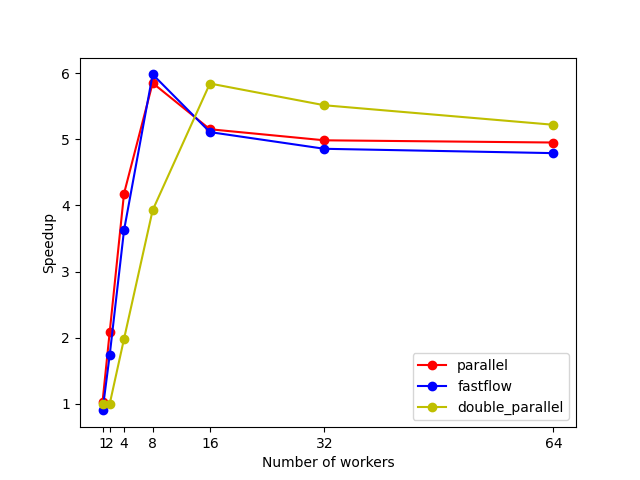
\includegraphics[width=200px, keepaspectratio]{imgs/speedup.png}
    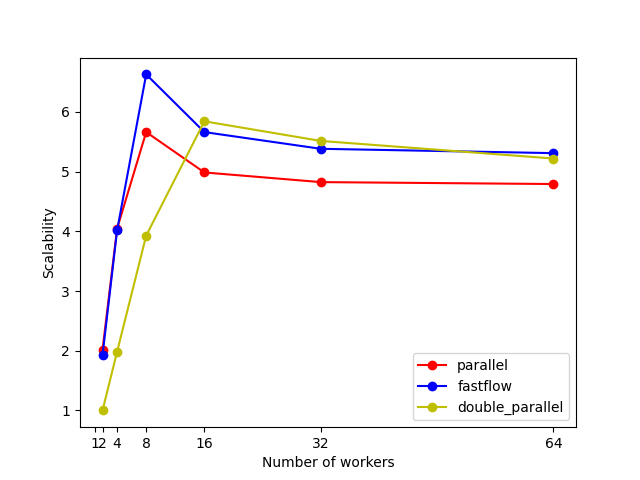
\includegraphics[width=200px, keepaspectratio]{imgs/scalability.png}
    \label{fig:speedup_scalability_plot}
\end{figure}


\begin{figure}[h!]
    \centering
    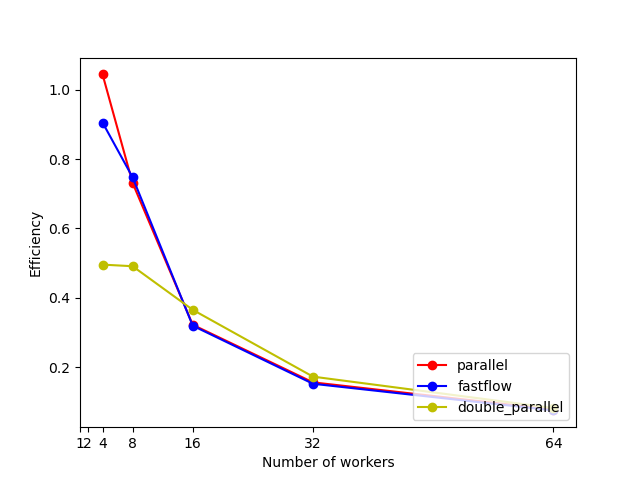
\includegraphics[width=200px, keepaspectratio]{imgs/efficiency.png}
    \label{fig:speedup_plot}
\end{figure}

\newpage
\subsection{Discussing the Results}
From the data it's clearly visible how the speedup, the scalability and the efficiency of the program are very constrained. In fact the speedup curve increases up to a factor of approximately $6$, decreases a bit and then remains constant. The first intuition that may occur is that this behaviour is caused by the increasing of the overhead produced by the number of threads in use. Even if this is obviously true, we can identify a stronger cause. If the overhead was the real problem in this case we should expect that the curve would have decreased when the number of threads was increased, but that's not really the case since the curve becomes pretty much a constant after the point of maximum speedup reached.\\
The main issue in this particular case is the cost of the sequential portion of the execution, which is very hard to overcome. As discussed in the Parallel Design section, parallelizing only the outer cycle doesn't require any synchronization on the data structure, however that means that the inner cycle -that in the results presented has length of $50'000$ iterations- will be computed entirely sequentially which, on the machine taken into consideration, it's an enormous effort. At the same time, parallelizing the inner cycle requires synchronization on the data structure and the overhead caused by that increases with the number of threads in use. Even in the case of the implementation that parallelizes both cycles, both problems appear.\\
There seems to be a very delicate trade-off between the amount of sequential work and the amount of overhead due to synchronization, that results in poor scalability and efficiency performances for all the solutions tested.\\
In other words, taking into consideration the Amdahl's law, we could say that the sequential portion of computation $f$ has a large enough impact on the computation to quickly overwhelm the benefits of parallelizing the portion $1-f$.

\subsection{Another possible approach}
Another solution that came to my mind to reduce as much as possible the sequential portion of the algorithm while lowering as much as possible the synchronization overhead was to use \texttt{std::unordered\_map} to store local minima found by the threads. This implementation would behave just like \texttt{double\_par.cpp}, with the exception that instead of using a \texttt{std::mutex} to synchronize the workers that compute the minima of a given point, the same workers would use a local minima data structure to obtain the $K$ local results and then add that data-structure to an \texttt{std::unordered\_map}. At the end of all the iterations that hashmap would contain $nw \times N$ data structures containing the local minima computed without the need of synchronization. Considering that a this point all the workers are free, it would be possible to assign to each worker a subset of points and in parallel merge the results stored in the hashmap. Then, as always, synchronize the output to the file.\\
This solution could get better performances in terms of scalability because: 
\begin{itemize}
    \item the pure sequential portion of code is limited to merging $nw$ \texttt{std::vectors} of size $K$ -which is typically very small, in the order of $10^1$-, which could imply huge benefits;
    \item the cost of the sequential portion of code is $\bigO(K \times N)$ where $N$ is the number of points assigned to each thread in the phase of merging the results, which is not very large since $K$ is typically very small and $N$ inversely proportional to the number of workers;
    \item in this case there's no synchronization on the data structure since the workers use local structures. One could argue that the access to the hashmap should be synchronized because they're not thread safe: even if that's true, inserting elements in parallel using different keys should never result in error, provided that the hash function is correct.   
\end{itemize}

Unfortunately I didn't have the time to realize a working implementation of the approach, hence I couldn't produce its results.

\section{Folder Overview \& Commands}
\subsection{Make and Running Benchmarks}
To make all the executable simply run \texttt{make} from \texttt{/SPM-Project}. To make only a specific executable please run:
\begin{itemize}
    \item \texttt{knn\_sequential} to build the executable of the sequential implementation;
    \item \texttt{knn\_parallel} to build the executable of the standard C!\verb++! implementation;
    \item \texttt{knn\_fastflow} to build the executable of the Fastflow implementation;
    \item \texttt{knn\_double\_parallel} to build the executable of the standard C!\verb++! implementation that parallelizes both cycles.
\end{itemize}
To compute the average time of execution please run navigate to \texttt{/SPM-Project/scripts} and run:
\begin{itemize}
    \item \texttt{sequential\_benchmark} to benchmark the sequential implementation;
    \item \texttt{parallel\_benchmark} to benchmark the standard C\verb!++! implementation;
    \item \texttt{fastflow\_benchmark} to benchmark the Fastflow implementation;
    \item \texttt{double\_benchmark} to benchmark the standard C\verb!++! implementation that parallelizes both cycles.
\end{itemize}
Please remember that \texttt{sequential\_benchmark} requires as parameters \texttt{number of iterations K [optional]input\_file} while all the other scripts require as parameters \texttt{number\_of\_iterations K number\_of\_workers [optional]input\_file}. Please keep in mind that -if specified- the \texttt{input\_file} must be present in \texttt{/SPM-Project/bin}.\\
To generate data please run \texttt{python3 /SPM-Project/scripts/generate\_data.py [optional] -n <\#points> -l <lower bound> -u <upper bound>}

\subsection{Folders content}
\begin{itemize}
    \item \texttt{bin} contains the executables and some useful pre-made input files;
    \item \texttt{data} contains output data and generated data;
    \item \texttt{fastflow} contains a local version of fastflow. In the folder received it's setup for my machine;
    \item \texttt{lib} contains useful libraries used in the implementations;
    \item \texttt{scripts} contains scripts to benchmark and generate new data;
    \item \texttt{src} contains the source of the implementations.
\end{itemize}

\end{document}